\documentclass{article}
\usepackage[english,activeacute]{babel}
\usepackage{listings}
\usepackage[latin1]{inputenc}
\usepackage{amsmath,amsfonts,amssymb,amstext,amsthm,amscd}
\usepackage{graphicx}
\usepackage{here} %usar el comandao[H] Para fijar la posición de las imágenes
\usepackage{multicol}
\graphicspath{{Imagenes/}}
% Estilo de página y encabezados 
% --------------------------------------------------------------------------------------------------------------------------------------------------------------
\usepackage{fancyhdr}
\setlength{\headheight}{15.2pt}
\usepackage[paperwidth=8.5in, paperheight=11.0in, top=1.0in, bottom=1.0in, left=1.0in, right=1.0in]{geometry}  
\pagestyle{fancyplain}
\fancyhead[R]{LRT2022 Digital design}
\fancyhead[C]{}
\fancyhead[L]{Fall 2024}
\fancyfoot[L]{}
\fancyfoot[C]{\thepage}
\fancyfoot[R]{}
% --------------------------------------------------------------------------------------------------------------------------------------------------------------
% Inicio del documento
\begin{document}
\fancypagestyle{plain}{
   	\renewcommand{\headrulewidth}{1pt}
   	\renewcommand{\footrulewidth}{1pt}
}
\renewcommand{\footrulewidth}{1pt}
\renewcommand{\tablename}{Tabla}
% --------------------------------------------------------------------------------------------------------------------------------------------------------------
%Titulo y autor
\author{}% No llenar, el documento debe ser anónimo..
\title{Individual assignment}
\date{LMT}%Escriba su carrera
\maketitle
% --------------------------------------------------------------------------------------------------------------------------------------------------------------
% Escribir resumen 150-200 palabras
\begin{abstract}
Este es el abstract.              
\end{abstract}

% --------------------------------------------------------------------------------------------------------------------------------------------------------------
\begin{multicols}{2} %Documento a dos columnas
\section{Introduction}\label{Intro}  
Digital electronics are the backbone of the technological society we live in today. This advancement has provided humanity with multiple benefits,
ranging from comunications to health care. The evolution of digital electronics has been marked by the devopment of numerous technologies
and methodologies that have revolutionized the way we process and transmit information. One of these improvements are the development of 
combinational logic circuits, which are fundamental components in digital systems. These circuits perform specific logical operations based on the combination of input signals,
providng the users with quick and efficient data processing capabilities, whithout the need for memory elements. Through the development of 
combinational circuits in the laboratory, we are able to understand and develop a deep understanding of the applications of digital electronics in various fields, such as computing, telecommunications, and control systems.

\section{Objectives}\label{Objectives}  
\begin{itemize}
  \item Design combinational logic circuits.
  \item Program and simulate custom combinational logic circuits in VHDL.
\end{itemize}
To achieve the objectives mentioned above, we must first understand the concepts of combinational logic circuits and the implementation in VHDL programming.
First and foremost, combinational logic circuits "are based on present inputs, and produces outputs that directly corresponds to the applied input signals." \cite{Joseph2025Hardware}. 
This means that the output of the circuit is determined solely by the current state of the inputs, without any memory or feedback elements involved.

\section{Methodology}\label{Meth}
The methodology applied in this laboratory practice was structured into three main phases: logical analysis, simulation in EDA Playground, and physical implementation on the Basys 3 board.

\subsection{Logical Analysis Phase}
During this first stage, the following activities were carried out:
\begin{enumerate}
    \item The truth tables and/or the functional requirements for each problem were analyzed and defined.
    \item Based on the truth tables or logical functions, the logic for the solution was laid out and optimized.
    \item Finally, the obtained results were documented for use in the subsequent simulation and programming phases.
\end{enumerate}

\subsection{EDA Playground Simulation Phase}
In the EDA Playground digital simulation environment, the following procedures were performed:
\begin{enumerate}
    \item The rock, paper and scissors game, water pump program, and coin detector circuits were programmed using the VHDL language.
    \item Testbenches were developed to verify the behavior of each circuit to prove certain behaviours of the code.
    \item The results obtained from the simulations were analyzed and compared with the previously developed truth tables and logic functions, ensuring the correct logical implementation of each design.
\end{enumerate}

\subsection{Basys 3 Board Implementation Phase}
Finally, the physical implementation of the circuits was carried out on the Basys 3 board, following the steps described below:
\begin{enumerate}
    \item The code for each circuit was synthesized, and the corresponding bitstream files were generated.
    \item Pin constraints (\texttt{.xdc} file) were assigned to map the logical signals to the physical components of the board (switches, LEDs, and displays).
    \item The designs were loaded onto the Basys 3 board, verifying their correct operation through practical input and output tests.
\end{enumerate}

\section{Results}\label{Results}
\subsection{Rock Paper Scissors Game}\label{R,P,S Game}
For the rock, paper, scissors game, the program was thougt out to have two players and a begin button, 
where each player could flip switches to select their choce. And once the play switch was raised, leds would light up to indicate
the winner of the game. For this circuit, the follwing truth table was developed:
\begin{table}[H]
\centering
\begin{tabular}{|c|c|c|c|c|}
\hline
\multicolumn{5}{|c|}{\textbf{Input}} \\
\hline
\textbf{PB} & \textbf{JAA} & \textbf{JAB} & \textbf{JBA} & \textbf{JBB} \\
\hline
1 & 0 & 0 & 0 & 0 \\
1 & 0 & 0 & 0 & 1 \\
1 & 0 & 0 & 1 & 0 \\
1 & 0 & 0 & 1 & 1 \\
1 & 0 & 1 & 0 & 0 \\
1 & 0 & 1 & 0 & 1 \\
1 & 0 & 1 & 1 & 0 \\
1 & 0 & 1 & 1 & 1 \\
1 & 1 & 0 & 0 & 0 \\
1 & 1 & 0 & 0 & 1 \\
1 & 1 & 0 & 1 & 0 \\
1 & 1 & 0 & 1 & 1 \\
1 & 1 & 1 & 0 & 0 \\
1 & 1 & 1 & 0 & 1 \\
1 & 1 & 1 & 1 & 0 \\
1 & 1 & 1 & 1 & 1 \\
\hline
\end{tabular}
\caption{Input Combinations for ent\_juego}
\label{tab:vhdl_juego_inputs}
\end{table}

\begin{table}[H]
\centering
\begin{tabular}{|c|c|c|}
\hline
\multicolumn{3}{|c|}{\textbf{Output (SAL)}} \\
\hline
\textbf{E} & \textbf{GJA} & \textbf{GJB} \\
\hline
0 & 0 & 0 \\
0 & 0 & 0 \\
0 & 0 & 0 \\
0 & 0 & 0 \\
0 & 0 & 0 \\
1 & 0 & 0 \\
0 & 0 & 1 \\
0 & 1 & 0 \\
0 & 0 & 0 \\
0 & 1 & 0 \\
1 & 0 & 0 \\
0 & 0 & 1 \\
0 & 0 & 0 \\
1 & 0 & 0 \\
0 & 1 & 0 \\
1 & 0 & 0 \\
\hline
\end{tabular}
\caption{Corresponding Outputs for ent\_juego}
\label{tab:vhdl_juego_outputs}
\end{table}

And based on these truth tables, a code was generated in VHDL to simulate and implement the circuit. The code is shown below:
\lstinputlisting[language=VHDL, caption=VHDL Code for Rock Paper Scissors Game, label=lst:vhdl_juego]{codigos/VHDL/PPT/design.vhd}
From which, the following testbench was created to verify the functionality of the code:
\lstinputlisting[language=VHDL, caption=VHDL Testbench for Rock Paper Scissors Game, label=lst:vhdl_tb_juego]{codigos/VHDL/PPT/testbench.vhd}
And the simulation on EDA Waves was generated as follows:
\begin{figure}[H]
	\centering
	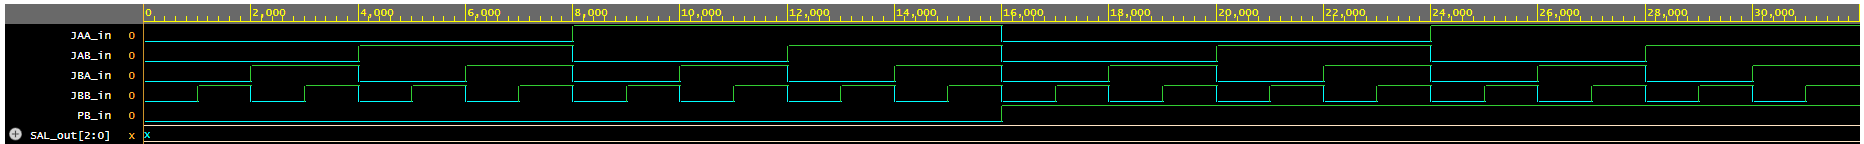
\includegraphics[width = 0.5\textwidth]{ppt.png}
	\caption{EDA Waves Simulation for Rock Paper Scissors Game}
	\label{fig:lab_ppt_eda}
\end{figure}
And finally, the circuit was implemented on the Basys 3 board, obtaining the following results:
\begin{figure}[H]
  \centering
  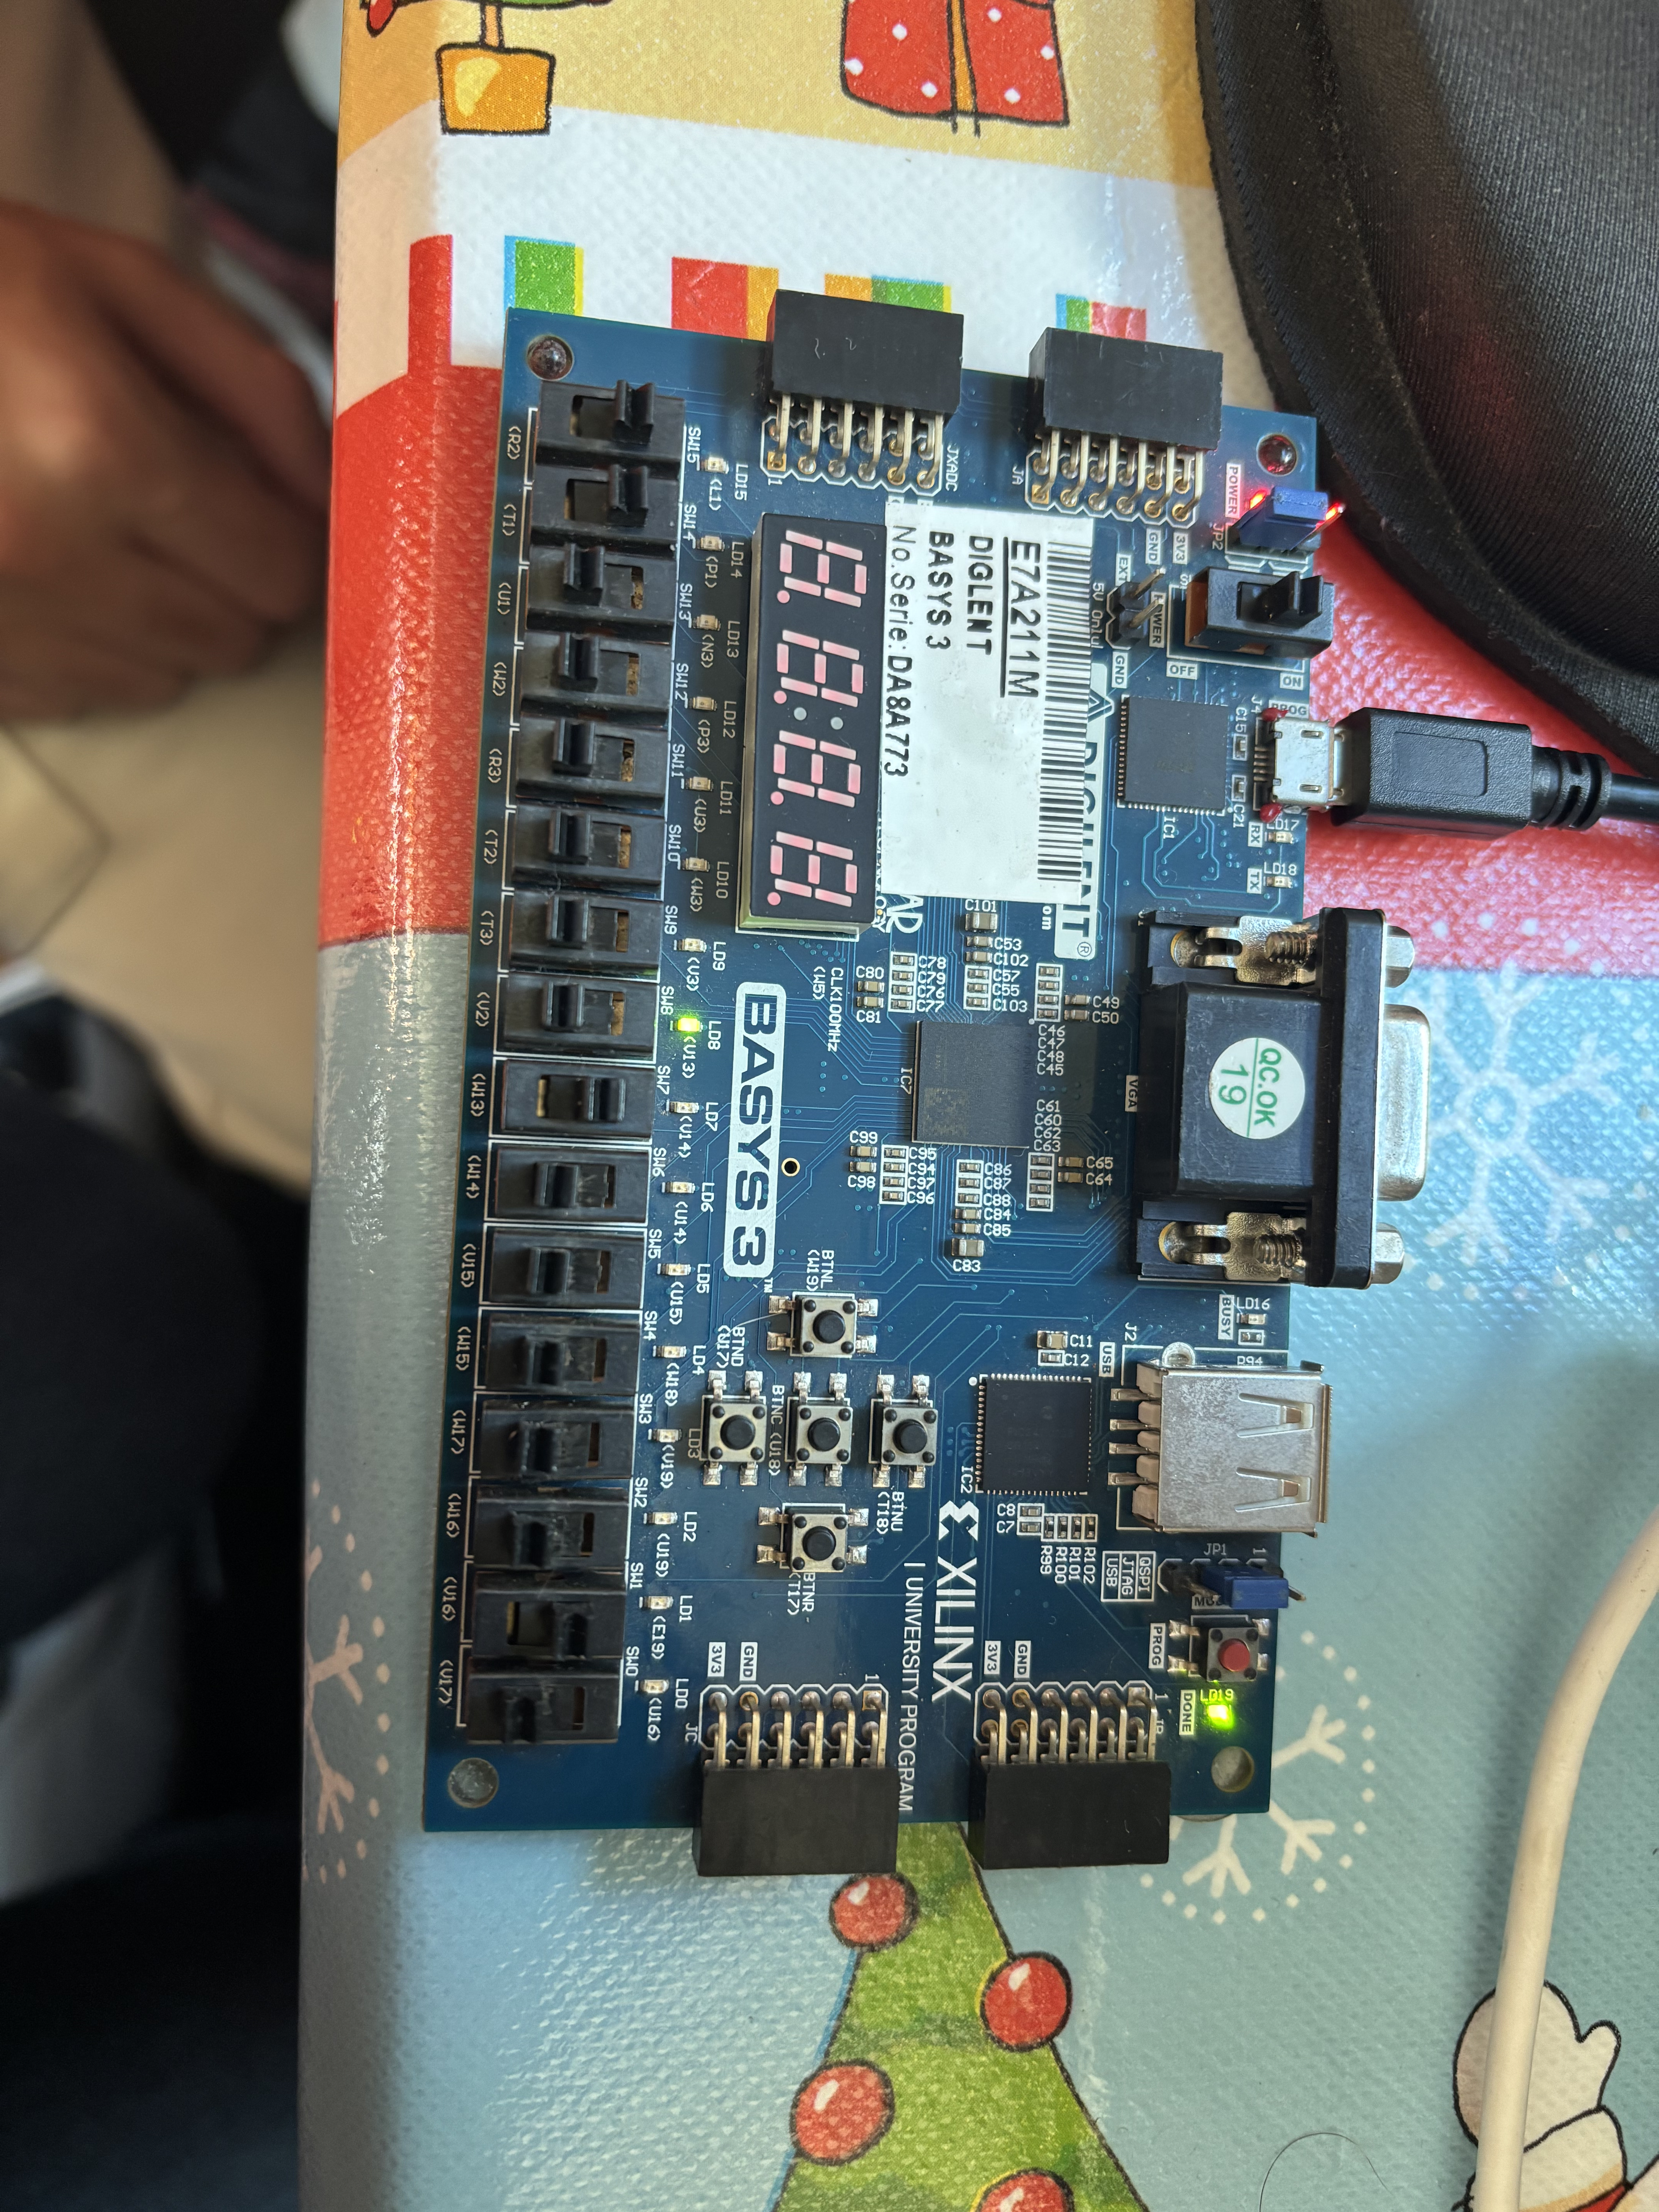
\includegraphics[width = 0.5\textwidth]{AWIN.jpg}
  \caption{Basys 3 Board Implementation for Rock Paper Scissors Game, A Wins}
  \label{fig:AWIN}
\end{figure}
\begin{figure}[H]
  \centering
  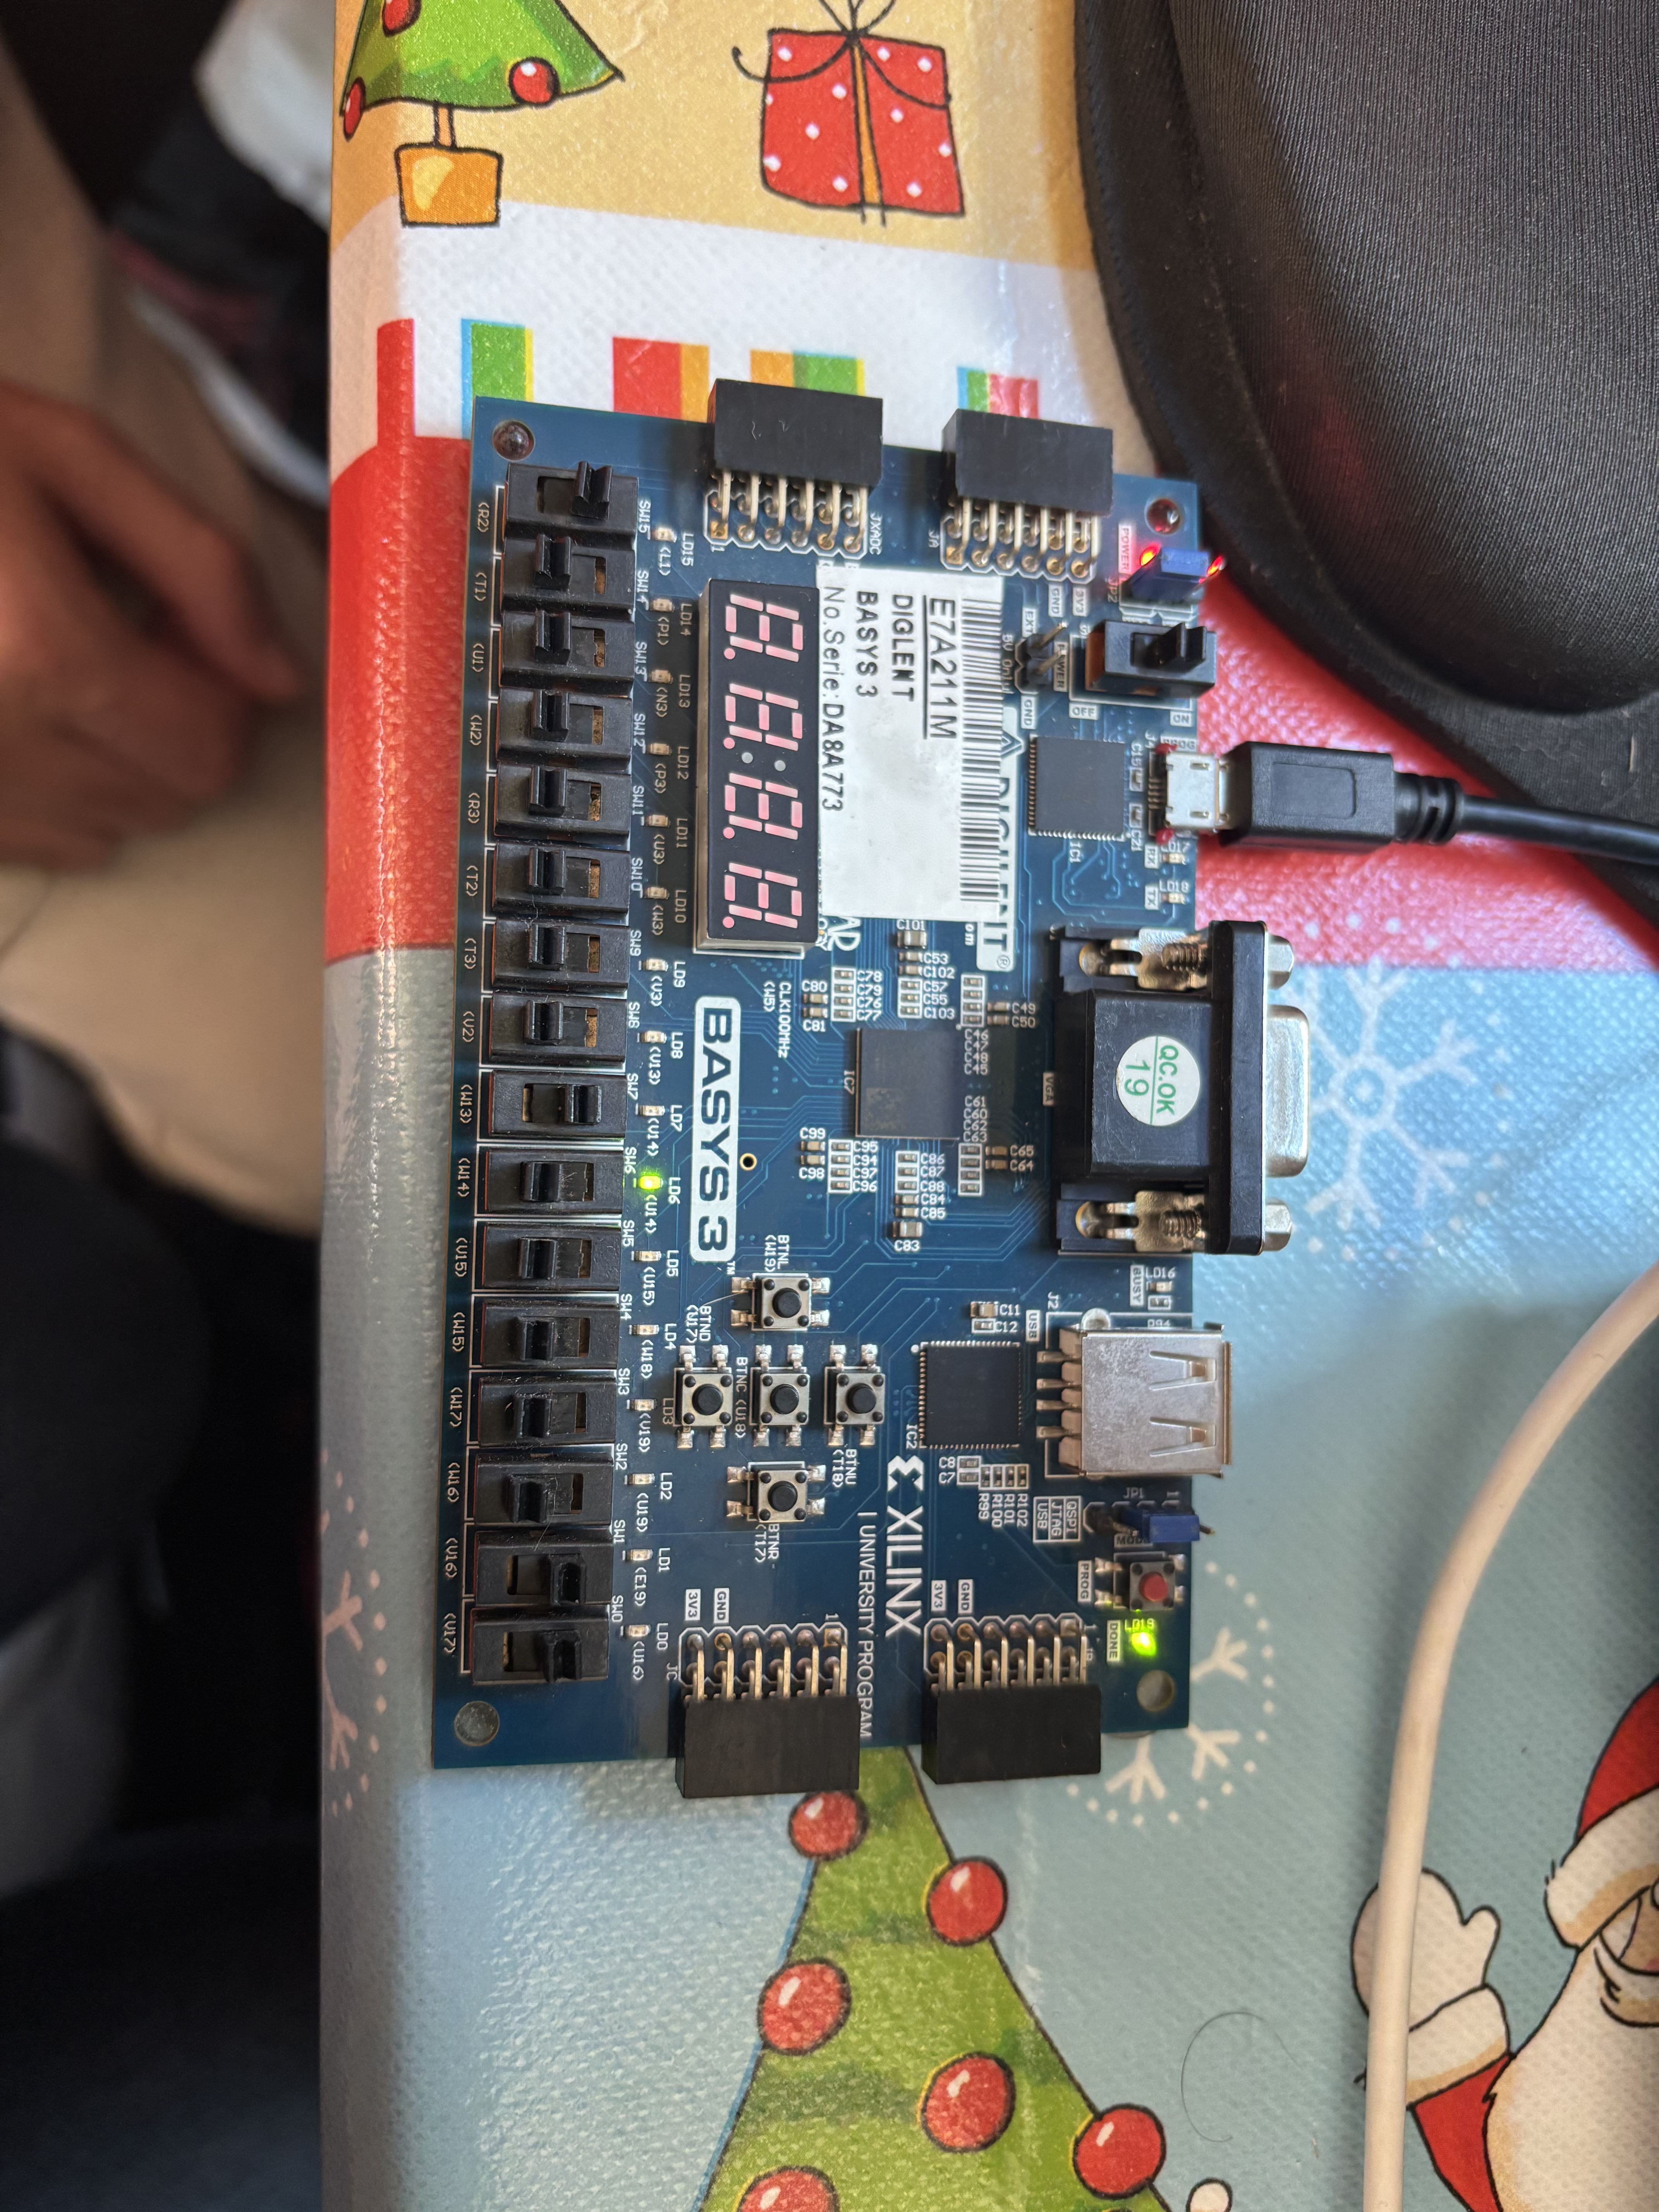
\includegraphics[width = 0.5\textwidth]{BWIN.jpg}
  \caption{Basys 3 Board Implementation for Rock Paper Scissors Game, B Wins}
  \label{fig:bwin}
\end{figure}
\begin{figure}[H]
  \centering
  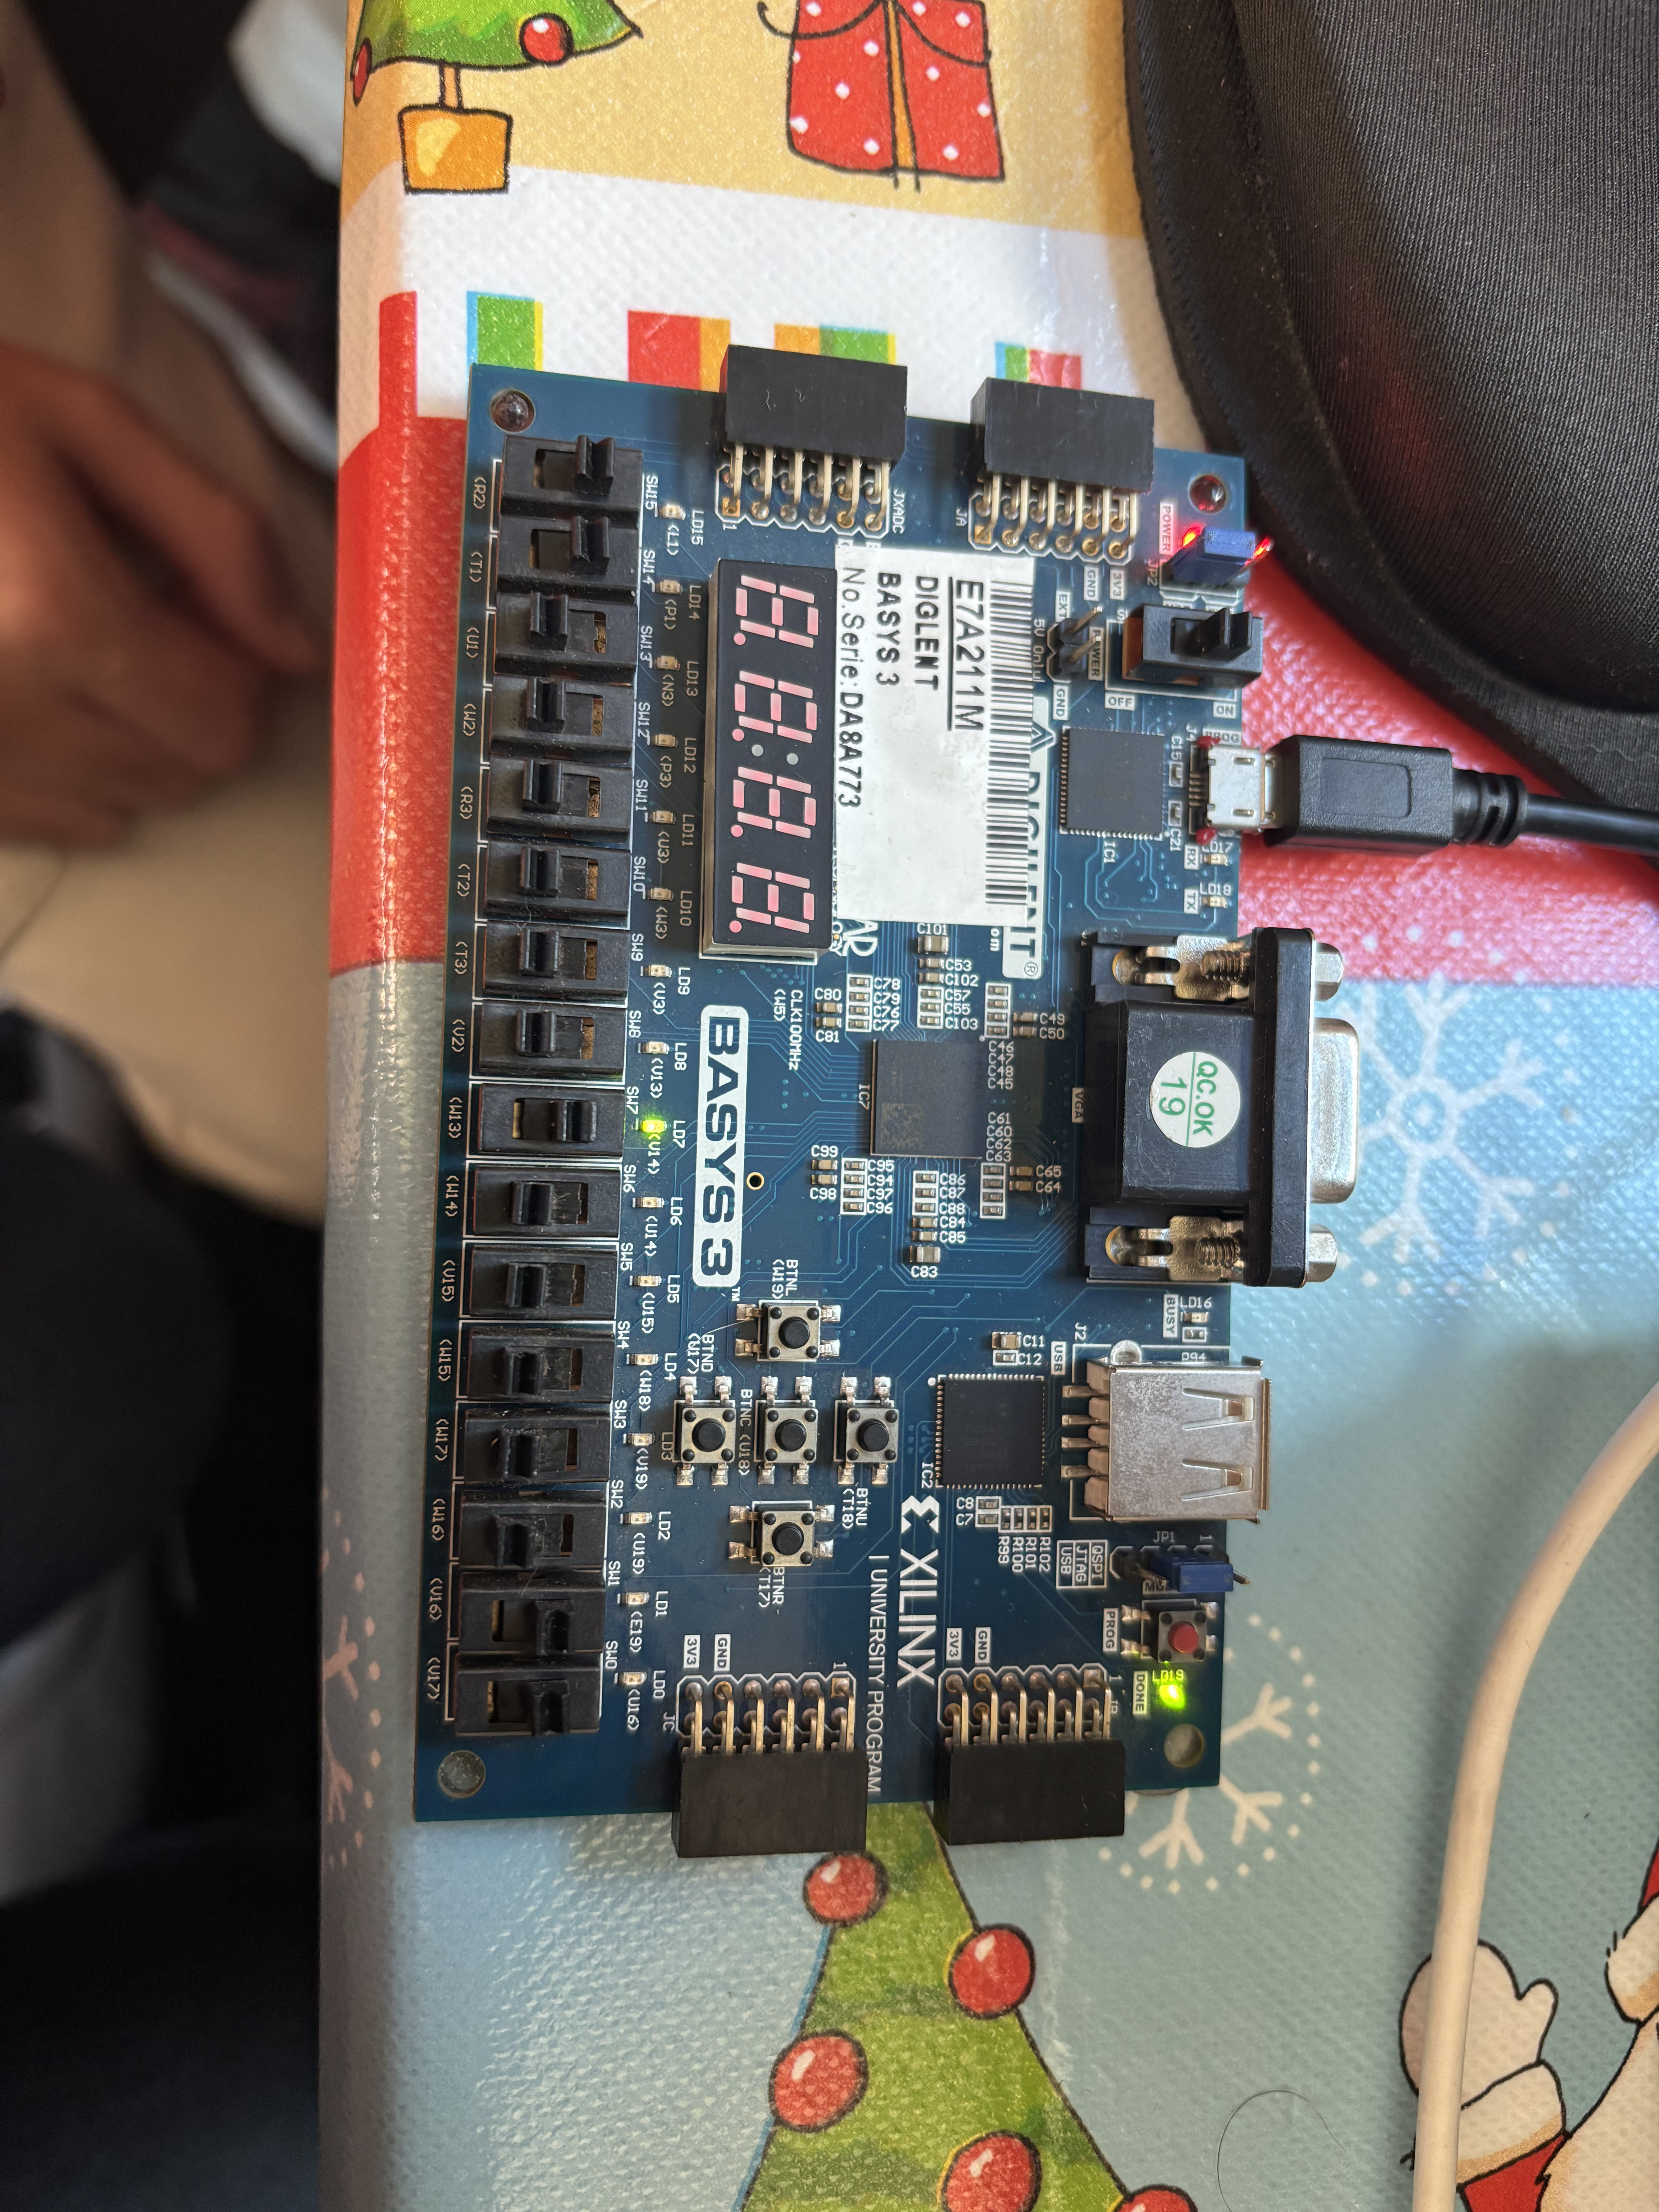
\includegraphics[width = 0.5\textwidth]{TIE.jpg}
  \caption{Basys 3 Board Implementation for Rock Paper Scissors Game, Tie}
  \label{fig:tie}
\end{figure}




% Bibliografía 
%---------------------------------------------------------------------------------------------------------------------------------------------------------------
\bibliographystyle{bst/IEEEtran} %Estilo de bibliografía NO MODIFICAR PARA MANTENER FORMATO
\bibliography{bib/bibliografia} %Fuentes bibliográficas Se recomienda utilizar un gestor de referencias (zotero, jabref, etc..)

% ----------------------------------------------------------------------------------------------------------------------------------------------------------------
\end{multicols}
\end{document}									
% Fin del documento